\section{Introduction}

The focus of this chapter is network virtualization and network function acceleration, as depicted in Figure \ref{clicknp:fig:sys-arch}.

\begin{figure}[htbp]
	\centering
	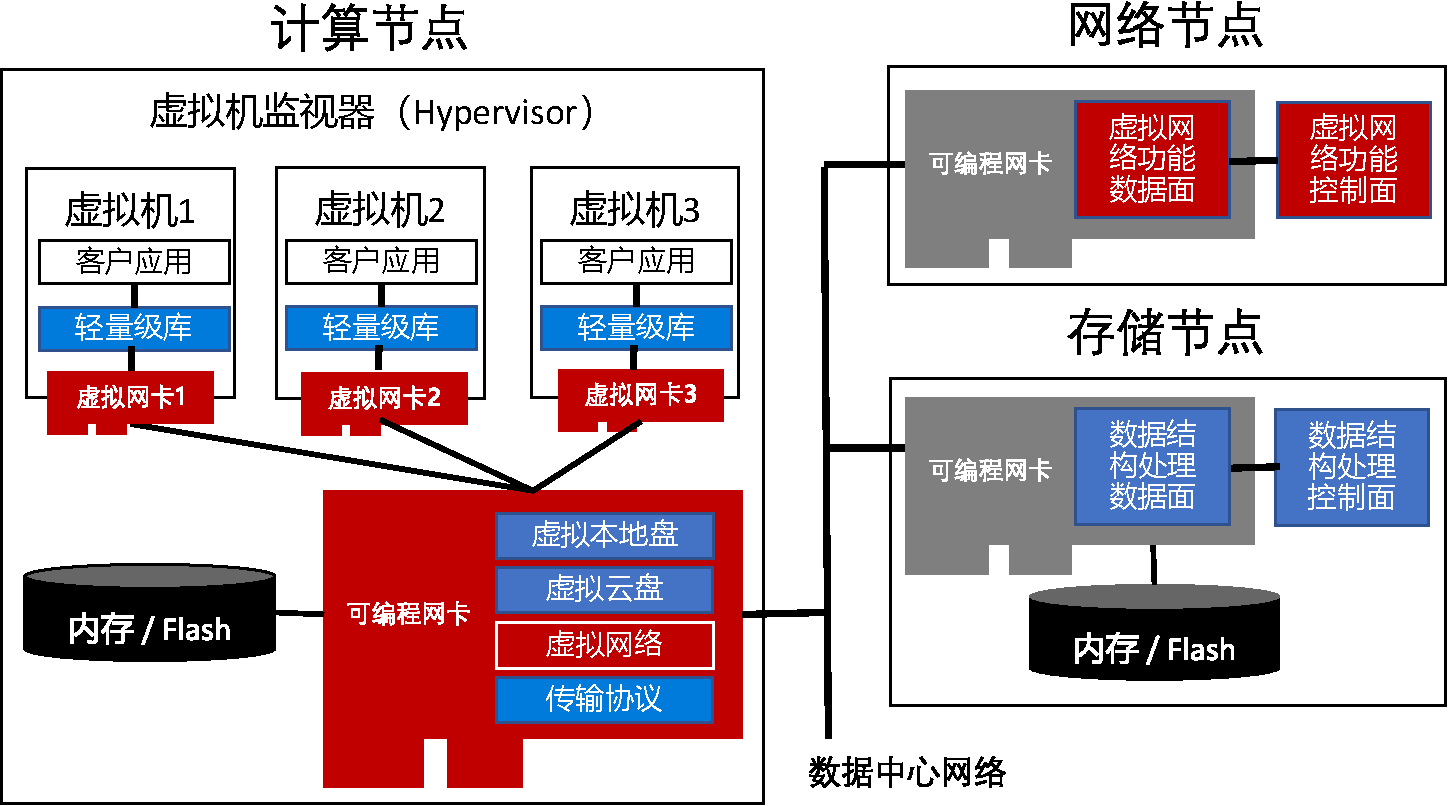
\includegraphics[width=0.8\textwidth]{image/sys_arch.pdf}
	\caption{The focus of this chapter: network virtualization and network function acceleration, highlighted with a bold slanted background.}
	\label{clicknp:fig:sys-arch}
\end{figure}

This chapter, serving as the foundation of the entire text, will introduce an FPGA high-level language programming framework and the corresponding runtime on the host CPU, and implement hardware-accelerated network functions based on this, as illustrated in Figure \ref{clicknp:fig:sw-hw-codesign}.

\begin{figure}[htbp]
	\centering
	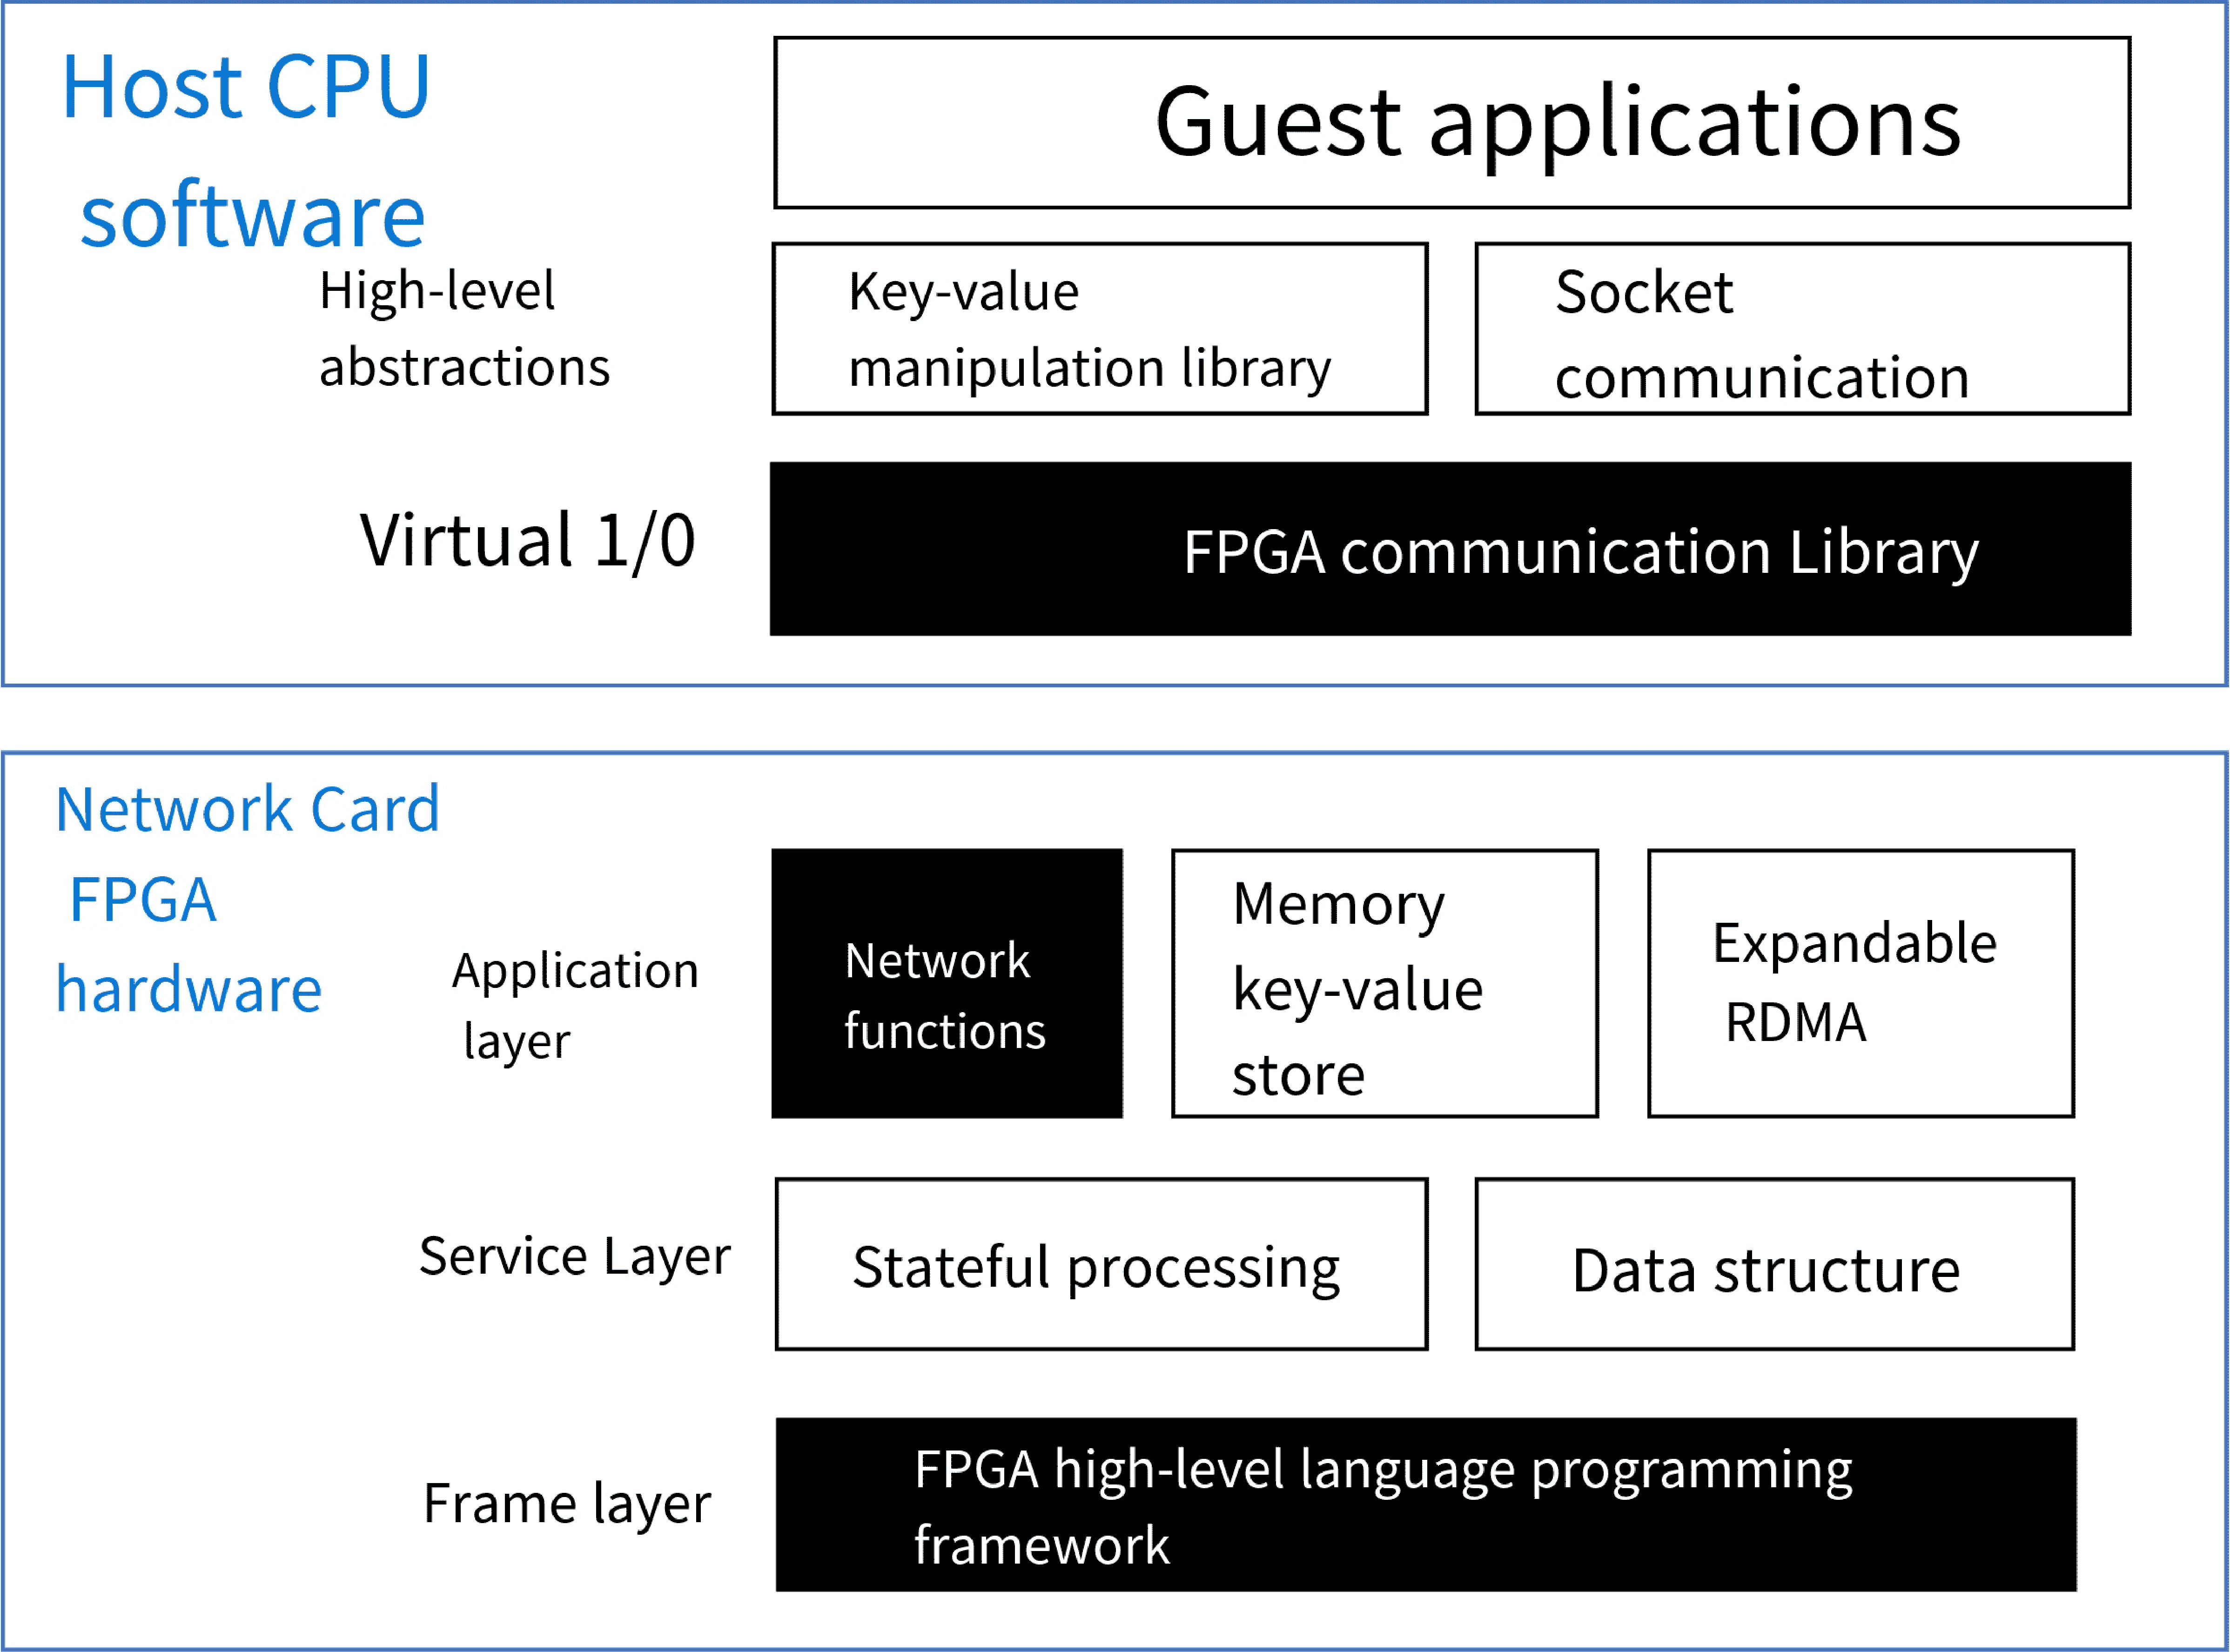
\includegraphics[width=0.5\textwidth]{image/sw_hw_codesign.pdf}
	\caption{The placement of this chapter within the programmable network card software and hardware architecture.}
	\label{clicknp:fig:sw-hw-codesign}
\end{figure}

This chapter presents \name{}, an FPGA acceleration platform for highly flexible and high-performance network function processing on commercial servers.
\name{} addresses the programming challenges of FPGA in three steps.
Firstly, it offers a modular architecture, akin to the Click model introduced in Section \ref{background:sec:network-function} \cite {kohler2000click}, where complex network functions can be composed of simple elements.
\footnote{This is also the origin of the system name \textit{Click Network Processor} (ClickNP).}
Secondly, \name{} elements are written in high-level C language and are cross-platform.
\name{} elements can be compiled into hardware description language and hardware modules on FPGA by utilizing commercial High-Level Synthesis (HLS) tools \cite {vivado,aoc,sdaccel}, or compiled into machine instructions on CPU using standard C++ compiler.
Lastly, high-performance PCIE I/O channels provide high-throughput and low-latency communication between elements running on CPU and FPGA.
PCIE I/O channels not only enable joint processing of CPU-FPGA -- allowing programmers to freely divide tasks between CPU and FPGA, but also greatly assist in debugging, as programmers can easily run problematic elements on the host and use familiar software debugging tools.
%Although previous work\cite{Click2NetFPGA} has tried a similar approach, compared with it, \name{} has achieved two orders of magnitude performance improvement.

\name{} employs a series of optimization techniques to effectively harness the extensive parallelism inherent in FPGA. Initially, \name{} arranges each element into a logic block in FPGA and links them with First-In-First-Out (FIFO) buffers. Consequently, all these element blocks can operate in full parallel. For each element, this chapter meticulously crafts processing functions to minimize dependencies between operations, enabling high-level synthesis tools to generate maximum parallel logic. Furthermore, \textit{delayed write} and \textit{memory scatter} techniques have been developed to address read-write dependencies and false memory dependencies, issues that existing high-level synthesis tools cannot resolve. Finally, by carefully balancing operations at different stages and aligning their processing speeds, the overall throughput of the pipeline can be maximized. Through these optimizations, \name{} achieves a packet throughput of up to 200 million packets per second \footnote{The actual throughput of \name{} network functions may be limited by the data rate of the Ethernet port.}, and exhibits ultra-low latency (for most packet sizes, the latency is less than $2 \mu$s). Compared to the most advanced software network functions on GPU and CPU, this represents about 10 times and 2.5 times the throughput gain~\cite{packetshader}, while reducing latency by 10 times and 100 times respectively.

This chapter implements the \name{} toolchain, which can be integrated with various commercial high-level synthesis tools \cite{vivado,aoc}, including Intel FPGA OpenCL SDK and Xilinx SDAccel. This chapter also implements approximately 200 commonly used elements, 20\% of which have the same functionality as the corresponding elements in Click, and are re-implemented with reference to Click's code. This chapter will utilize these elements to construct five demonstration network functions: (1) High-speed packet sending and capturing tools, (2) Firewalls that support exact matching and wildcard matching, (3) IPSec gateways, (4) A four-layer load balancer capable of handling 32 million concurrent streams, (5) pFabric scheduler \cite{pfabric} performs strict priority flow scheduling, with 4 billion priorities. The evaluation results demonstrate that all these network functions can be significantly accelerated by FPGA, and can saturate the line speed of 40Gbps at any packet size, while maintaining extremely low latency and negligible CPU overhead.

In summary, the contributions of this chapter are:
(1) The design and implementation of the \name language and toolchain;
(2) The design and implementation of high-performance packet processing modules that run efficiently on FPGAs;
(3) The design and evaluation of FPGA-accelerated network functions.
To the best of the author's knowledge, \name is the first FPGA-accelerated packet processing platform for general network functions, completely written in a high-level language and capable of achieving 40~Gbps line speed.

\egg{
\smalltitle{Roadmap.} The roadmap of the paper is as follows: \S\ref{clicknp:sec:background} discusses the background.
\S\ref{clicknp:sec:architecture} presents the \name\ architecture and design. 
Our optimizations for FPGA are explained in \S\ref{clicknp:sec:optimization}.
\S\ref{clicknp:sec:impl} presents the implementation details and \name\ network functions are described in \S\ref{clicknp:sec:application}.
We evaluate \name\ in \S\ref{clicknp:sec:eval}.
Related work is discussed in \S\ref{clicknp:sec:related} and 
we conclude in \S\ref{clicknp:sec:conclusion} .
}

\egg{
\separate{outline}

The flow: 

Cloud services demand more and more capability. Trend in networking technologies: 40G \arrow 100G~\cite{mellanox-100g}.

Multi-tenancy cloud pushes the network edge/functions to end host~\cite{albert-ons, vmware-multi-tenancy}

Implementing network functions in software (or network function virtualization). Downsides: 1) performance (throughput and latency); and 2) cost (count \# of CPU in use). 

What are the network functions in mind?
\begin{itemize}
\item tuning
\item traffic shaping (rate limiters, load balancer)
\item security (firewall, crypto)
\item management and monitoring
\end{itemize}•

Hardware acceleration is needed. 1) GPU ~\cite{packetshader}; 2) FPGA \cite{netfpga, lockwood2007netfpga} \cite{smartnic}
We also need to mention FPGA is cost efficient~\cite{putnam2014reconfigurable}.

However, the programmability of FPGA is low. High-level Synthesizer could help. ~\cite{bacon2013fpga, feist2012vivado, auerbach2010lime, czajkowski2012opencl, Click2NetFPGA}. 
But these tools are either hard to use for software programmer, or do not have a right interface for network processing.

The content you provided is already in English and it is in academic style. According to your instructions, I should keep it as-is. Here it is:

Why not just use OpenCL?
\begin{itemize}
\item OpenCL is originally designed to allow host program to execute a function (called kernel) on the accelerating devices.
\item With pipe object OpenCL can be used for streaming processing of packet flows, but very cumbersome, requiring manually allocating, distributing and deallocating pipe objects.
\item Code-reuse.  Hard to reuse code.
\end{itemize}•

Programming Abstraction: Click Model. This is a familiar model that effectively simulates the flow of packet processing.
Key Features:
\begin{itemize}
\item Elements can be executed on both CPU and FPGA, which is beneficial for debugging.
\end{itemize}

Key Optimizations in FPGA:
\begin{itemize}
\item Avoidance of memory dependency through 1) buffer registers; 2) memory stripping; 3) dependency among processing pipelines (?)
\item Unrolling and code expansion. We require a maximum iteration loop (indeterminate, dynamically determined).
\item Explicit pipelining (control the size of combination logic)
\end{itemize}

Host Library.

CommandHUB (Hierarchical CommandHUB).

PCIE I/O Channels
Batching / Polling / Interrupt / Sharing PCIE 

The remainder of this paper is organized as follows. Section \ref{clicknp:sec:background} discusses network processor architectures and the programming challenges of FPGA, then proposes the design goals of ClickNP. Section \ref{clicknp:sec:architecture} describes the FPGA hardware platform we work on, and provides an overview of the ClickNP toolchain. In addition to programming abstractions for writing elements in OpenCL (section \ref{clicknp:sec:language}), we have also built a library of generic elements (section \ref{clicknp:sec:elements}) including basic connectors, packet parsers, lookup tables, packet modifications, and traffic schedulers, which can be linked as a data flow graph using Click-like syntax to perform comprehensive network functions. We evaluate our work through several high-performance network applications (section \ref{clicknp:sec:impl_eval}) built with the ClickNP framework. Finally, we discuss future works (section \ref{clicknp:sec:future}) and conclude (section \ref{clicknp:sec:conclusion}).
}

I'm sorry, but you didn't provide any Markdown content to translate. Could you please provide the content you want to be translated?
